% GRASP: Copyright 1997,1998,1999  Bruce Allen
% $Id: man_testmass.tex,v 1.5 1999/07/11 21:22:17 ballen Exp $
%
% GRASP Routines: Waveforms from perturbation theory
% Author: S.Droz (droz@physics.uoguelph.ca)
%
%
% $Id: man_testmass.tex,v 1.5 1999/07/11 21:22:17 ballen Exp $
%
% $Log: man_testmass.tex,v $
% Revision 1.5  1999/07/11 21:22:17  ballen
% Added RCS id strings
%
% Revision 1.4  1998/10/05 19:14:54  ballen
% Updated manual to use new hyperref package.
%
% Revision 1.3  1998/06/06 20:43:28  ballen
% Serge modified manuals, and added figure.
%
% Revision 1.5  1998/04/01 22:02:24  droz
% This is the version in GRASP 1.6.5.
%
% Revision 1.3  1998/02/25 21:44:15  droz
% All routines and the error messages are now documented.
% We still need to add the examples and correct all the errors.
%
% Revision 1.2  1998/02/24 22:11:31  droz
% Most routines are now documented.
%
% Revision 1.1  1998/02/23 22:02:10  droz
% Initial revision
%
%
 \DeclareRobustCommand{\nicefrac}[2]{\hspace{0.1em}%
  \raisebox{0.5ex}{${\scriptstyle
#1}$}\hspace{-0.1em}/\hspace{-0.07em}%
  \mbox{${\scriptstyle #2}$}}
\section{GRASP Routines: Waveforms from perturbation theory}
\label{s:BHPT}
\setcounter{equation}0
An alternative method of calculating the waveforms generated during a binary
inspiral is provided by black hole perturbation theory.
In the limit of a small mass ratio $\eta = \nicefrac{m_1 m_2}{(m_1 + m_2)^2}$ (the
test mass limit) we can treat the effects of the smaller body as perturbations of
the gravitational field of the larger mass. If the latter is a black hole then
the Teukolsky formalism \cite{teukolsky:1973} can be used to calculate these perturbations.
The corrections to 
the metric are then expressed as an infinite sum over multipole 
moments. Here we will consider the case of a Schwarzschild black hole.

\subsection{The waveform}

The Teukolsky formalism gives the two components $h_+$ and $h_\times$ of the
gravitational waves produced by a test mass in a fixed, circular orbit of radius $r_0$
 as
\begin{equation}
  h_+(u) - i h_\times(u) = \frac{2 G \mu}{r c^2} \sum_{l\geq 2, |m| \leq l}
            A_{lm}(M \Omega) e^{-i m \Omega (t - c r^*)} {}_{-2}Y_{lm}(\vartheta,
                        \varphi),
        \label{e:wave1}
\end{equation}
where  $u=t-c r^*$ is the standard retarded time. Here $G$ is Newton's constant and
$c$ the speed of light.
Here the functions ${}_{-2}Y_{lm}(\vartheta,\varphi)$ are the spherical harmonics
of spin weight $-2$, $\Omega$ is the angular velocity and $M=m_1+m_2$ is the
total mass of the system. 
The angles $\vartheta$ and $\varphi$ are the usual spherical coordinates, as defined in
Section \ref{ss:Quasimodo}, Figure \ref{f:orient} ($\vartheta = \iota$ and $\vartheta = \beta$). Since the
motion is symmetric around the $z$-axis $\varphi$ does not have an intrinsic meaning.
Throughout this section angles are measured in radians.
The amplitudes $A_{lm}$ are constants and have to be
calculated numerically by solving the Teukolsky equation.
We provide $A_{lm}$ tabulated in a datafile \cite{ericsfiles} as a function of
the orbital velocity $v$ (measured in units of the speed of light $c$)
\begin{equation}
  c v = r_0 \Omega = \sqrt{\frac{G M}{r_0}} = (G M \Omega )^\frac{1}{3} 
  = (2 \pi G M f)^{\frac{1}{3}}.
\end{equation}
Here $f$ is the {\em orbital} frequency measured in units on Hertz. 

To account for the decay of the orbit due to the emission of gravitational waves
we use an adiabatic approximation: The energy radiated away as calculated from
expression  (\ref{e:wave1}) is used to calculate the change in 
orbital frequency.
By doing so, $\Omega$, and thus also $v$, become functions of time and we
have to replace the product $\Omega u$ by an integral 
$\int \Omega(u) du$.

Following \cite{droz97} we find that the time evolution of the velocity is 
governed by 
\begin{equation}
  \dot{v} = \frac{32}{5} \frac{\mu c^3}{G M^2} v^9 \frac{P(v)}{Q(v)}, 
  \label{e:vdot}
\end{equation}
where $\mu = \nicefrac{m_1 m_2}{M}$  is the reduced mass of the system.
The function $P(v)$, which is determined by the $A_{lm}$'s,  is defined 
by
the equation
\[
  \dot{E} = \frac{dE}{dt} = P(v) \left(\frac{dE}{dt}\right)_N
\]
where $(dE/dt)_N = \nicefrac{-32 \mu^2 v^{10} c^4}{5 G M^2}$ is the  quadrupole-formula
expression for the gravitational-wave luminosity.
We also provide $P(v)$ in tabulated form \cite{ericsfiles}. The function $Q(v) =
(1-6v^2)(1-3v^2)^{-\frac{3}{2}}$ relates the energy and frequency of the
orbiting particle:
\[
   \frac{dE}{df} = E(v) \left(\frac{dE}{df}\right)_N.
\]
This can be calculated by solving the geodesic equation for
circular orbits in the Schwarzschild spacetime.

Note that $v(t)$ can be calculated from equation (\ref{e:vdot}) once and for
all:
First (numerically) calculate the solution $V(t)$ of equation (\ref{e:vdot}) with
the factor $\nicefrac{\mu c^3}{G M^2}$ set to one; then the solution $v(t)$ for general $\mu/M^2$ is
simply
\begin{equation}
  v(t) = V\left(\frac{\mu c^3}{G M^2} t\right).
  \label{e:vot}
\end{equation}  
As mentioned before, we have to replace the product $\Omega u$ in equation (\ref{e:wave1}) by
an appropriate integral. We first note that we want to look at waves at a fixed
radius $r^* \rightarrow \infty$. We can thus simply ignore the dependence on 
$r^*$ because it will only contribute a fixed phase $\varphi_0$. Since 
our data are
tabulated as functions of the orbital velocity $v$, it is convenient to use $v$
instead of the time $t$ as an independent variable. This is permissible 
because
$v$ depends monotonically on $t$. Thus the phase becomes:
\begin{equation}
  -i m \Omega t \ \ \longrightarrow \ \ -i m \frac{M}{\mu} \frac{5}{32}
  \int_{v_0}^v dv' \frac{Q(v')}{P(v') v'^6} =: -i m \frac{M}{\mu} \Phi(v_0,v).
  \label{e:Phi}
\end{equation}
It is important to note that $\Phi$ is {\em not} unique, but depends on
an arbitrary parameter $v_0$. As with $r^*$, a change in $v_0$ will only
affect the phase $\varphi_0$. Since $\Phi$ can become rather large, the
freedom in choosing $v_0$ can be used to keep $\Phi$ small in the region
of interest.  A good choice of $v_0$ will improve the numerical accuracy
tremendously.  (For example, the standard trigonometric functions in C
become hopelessly inaccurate for arguments  $> 10^6$ for floats and $>
10^{10}$ for doubles).

The signal is now given by
\begin{equation}
  h_+(t) - i h_\times(t) = \frac{2 G \mu}{r c^2} \sum_{l\geq 2, |m| \leq l}
            A_{lm}(v(t)) e^{- i m \frac{M}{\mu} \Phi(v_0, v(t))} {}_{-2}Y_{lm}(\vartheta,
                        \varphi),
        \label{e:wave2}
\end{equation}
where $v(t)$ is given by equation (\ref{e:vot}). 

To extract $h_+$ and $h_\times$ independently  we use the fact that
$A_{l-m} = (-1)^l \overline{A}_{lm}$ and, since ${}_{-2}Y_{lm}(\vartheta, 
\varphi) = {}_{-2}Y_{lm}(\vartheta,0)\, e^{i m \varphi}$
and ${}_{-2}Y_{lm}(\vartheta,0)$ is real, we have
${}_{-2}Y_{l-m}(\vartheta, \varphi)= {}_{-2}Y_{lm}(\vartheta,0)\, 
e^{-i m \varphi}$ \cite{goldberg:1967}.
We can now split the sum (\ref{e:wave2}) into real and imaginary 
part. This gives the two components as
\begin{eqnarray}
  h_+ =  \frac{2 G \mu}{r c^2} \sum_{2 \leq l, 1 \leq m \leq l }
     \left(c_m \,  \Re_{lm} - s_m \,  \Im_{lm} \right) 
     \left({}_{-2}Y_{lm}(\vartheta,0) + (-1)^l 
     {}_{-2}Y_{l-m}(\vartheta,0)\right) \nonumber \\
     {} \label{e:hphc} \\
     h_{\times} =  \frac{2 G \mu}{r c^2} \sum_{2 \leq l, 1 \leq m \leq l}
     \left(s_m \, \Re_{lm} + c_m \,  \Im_{lm} \right) 
     \left(-{}_{-2}Y_{lm}(\vartheta,0) + (-1)^l 
     {}_{-2}Y_{l-m}(\vartheta,0)\right). \nonumber
\end{eqnarray}
Here we have introduced the notation $\Re_{lm} := {\rm Re}\, A_{lm}$, 
$\Im_{lm} := {\rm Im}\, A_{lm}$ and $s_m := \sin(-m (\Phi M/\mu  - \varphi))$ 
and $c_m := \cos(-m (\Phi M/\mu  - \varphi))$.


The GRASP routine which calculates $h_+$ and $h_\times$ uses 
expression (\ref{e:hphc}) truncated to a finite number of terms 
determined by the user.
Finally we note that a change in $\varphi$ has the same effect on the 
waveforms as a change in $r^*$ and $v_0$.

\subsection*{A note on the allowed frequency range}

The frequency range of a signal calculated from black hole 
perturbation theory is bounded from above by the  
innermost stable circular orbit. This corresponds, by virtue of 
equation (\ref{e:vdot}), to an orbital velocity of $v_{\rm max} = 
\nicefrac{1}{\sqrt{6}}$. In practice there is also a lower bound. Since 
zero frequency would correspond to an infinite orbital radius we have 
to introduce a cutoff. In the present data files $v_{\rm min} \simeq
 0.0395$. Figure \ref{f:frange} shows the allowed frequency range as 
 a function of the total mass $M$.
 

\begin{figure}[h]
\begin{center}
\epsfig{file=Figures/fig_frange.ps,angle=-90,width=6in}
\caption{ \label{f:frange}
Maximum and minimum orbital frequencies as a function of the total mass
$M / M_\odot$ of the system.}
\end{center}
\end{figure}


Since $\dot{v}$ in equation (\ref{e:vdot}) diverges at $v=v_{\rm 
max}$ calculating $v(t)$ at the upper limit is numerically difficult. 
However this is not a problem in the time domain, since the system spends very little time near $v =
v_{\rm min}$. An value 
of $f_{\rm max}$ inaccurate by several percent will typically not change 
the signal by  even one wave cycle. 

\subsection{Chirp generation for test mass signals}

The routines provided in this package were designed to resemble as 
closely as possible the chirp generating routines for post-Newtonian 
signals. However, because of the different functional forms for  the two 
types of waveforms some differences where unavoidable.

The main routine is {\tt testmass\_chirp()} which returns
$h_+$ and $h_\times$ in a given frequency 
interval. However, before being able to use {\tt testmass\_chirp()}, one 
has to read in the data files, calculate the phase $\Phi(v_0,v)$, etc.
There are a number of routines provided that allow one to perform
these tasks with a minimum of amount of work.

For {\tt testmass\_chirp()} to work, the program must make sure that the
two data files containing the mode amplitudes $A_{lm}(v)$ and the luminosity $P(v)$
have been read. It then has to calculate 
$V(t)$ (which can be inverted to give $t(V)$) and 
$\Phi(v_0,v)$. Furthermore, it has to make the number of data points
known to the package, in order for the interpolation routines
to work. The package currently assumes that all data files have the same
number of points and that $v$ is equally spaced. 
Note that all the functions in the package take the orbital frequency 
$f= \nicefrac{v^3 c^3}{G M \pi}$, instead of $v$, as input. 
\clearpage
%%%%%%%%%%%%%%%%%%%%%%%%%%%%%%%%%%%%%%%%%%%%%%%%%%%%%%%%%%%%%
%
% testmass_chirp
%
%%%%%%%%%%%%%%%%%%%%%%%%%%%%%%%%%%%%%%%%%%%%%%%%%%%%%%%%%%%%%

\subsection{Function: {\tt testmass\_chirp()}}
\setcounter{equation}0
{\tt 
int testmass\_chirp(float m1, float m2, float theta, float phi,
               float *Phase, float f\_start, float f\_end, float *f\_started,
               float *f\_ended,  float dt, float **hplus, float **hcross, 
	       float **frequency, int *number\_of\_points, int MaxL, int *modes)}\\
This function calculates the two unnormalized signals $h_+$ and
$h_\times$. To normalize just multiply the output
by the prefactor $2 \mu/r$. This is the main routine of the test mass package.
The arguments are:
\begin{description}
\item{{\tt m1}}: Input.  The mass of the first body in units of the solar mass.
\item{{\tt m2}}: Input.  The mass of the second body in units of the solar mass.
\item{{\tt theta}}: Input. The inclination angle $\vartheta$ in radians.
\item{{\tt phi}}: Input. The azimuth  $\varphi$ in radians.
\item{{\tt Phase}}: Input: A pointer to an array containing the
           phase function $\Phi(f_0,v)$. The number of points calculated 
		   must have been set beforehand, either by the supplied routines or
		   through an explicit call of {\tt Set\_Up\_Data()}.  
\item{{\tt f\_start}}: Input. Starting {\em orbital} frequency in Hertz.
       If the frequency is too low it will be adjusted to the minimum allowed
	   frequency.
\item{{\tt f\_end}}: Input. Final {\em orbital} frequency in Hertz. 
       If set too high the program will terminate at the maximum 
	   frequency.
\item{{\tt f\_started}}: Output. The frequency in Hertz where the chirp actually
                   started. This is max$(f_{\rm start}, v_{\rm min}^3 c^3/(2 \pi G M))$.
\item{{\tt f\_ended}}: Output. The frequency in Hertz where the chirp terminated.
               This is min$(f_{\rm end}, v_{\rm max}^3 c^3/(2 \pi G M))$
\item{{\tt dt}}: Input. The time interval between successive samples in
seconds.
\item{{\tt hplus}}: Input/Output. The signal $h_+$ is stored in the
    array {\tt *hplus[0..number\_of\_points-1]}. If {\tt **hplus == NULL}
	memory will be allocated, otherwise the user has to provide the memory.
	The allocated memory is given by {\tt ((number\_of\_points/kNumberOfFloats
	+1)*kNumberOfFloats*sizeof(floats)}. Note that this performs integer
	arithmetic, so it's not what you might expect.
\item{{\tt hcross}}: Input/Output. The signal $h_\times$ is stored in the
    array {\tt *hcross[0..number\_of\_points-1]}. If {\tt **hcross == NULL}
	memory will be allocated, otherwise the user has to provide the memory.
	Use the same expression as above to get the memory allocated.
\item{{\tt frequency}}: Input/Output. The orbital frequency $f(t)$ is stored in
    the array {\tt *frequency[0..number\_of\_points-1]}. If {\tt **frequency == NULL}
	memory will be allocated, otherwise the user has to provide the memory.
\item{{\tt number\_of\_points}}: Input/Output. The number of points requested.
   If {\tt number\_of\_points == 0} then memory will be allocated for you.
   If {\tt number\_of\_points} is nonzero, then at most this number of points will 
   be returned. You must give the number of points if you allocated memory for
   any of the arrays {\tt hplus}, {\tt hcross} or {\tt frequency}
   yourself. On exit this variable holds the actual number of points calculated.  
\item{{\tt MaxL}}: Input. The maximum number of modes to be used. For the
supplied data file this has to be less than or equal to five. It is assumed that all
$m$'s are available for a given $l$. 
\item{{\tt modes}}: Input. An array containing a list of  modes to include in the
sum (\ref{e:wave1}). The array contains $1$'s for modes to be included
and $0$'s otherwise. The sequence of modes is \\
\begin{center}
\begin{tabular}{|l|ccccccccccccc|}
\hline
index &  0 &  1 &  2  & 3 & 4  &  5 &  6 &  7 &  8 &  9 & 10 & 11 &\ldots \\ \hline
l     &  2 &  2 &  2 &  2 & 3  &  3 &  3 &  3 &  3 &  3 & 4  & 4 & \ldots \\ \hline
m     & -2 & -1 & +1 & +2 & -3 & -2 & -1 & +1 & +2 & +3 & -4 & -3 &\ldots \\ \hline
\end{tabular}\\
\end{center}
Use the macro \\
{\tt \#define mode2(l,m)  ((l)*(l) + m - 2 - ((m > 0) ? 1 : 0))}
to calculate the index.

\item{Return value}: Output. {\tt testmass\_chirp()} returns $0$ if there was
   no error, and an error code otherwise. These codes are described in Section \ref{tm:errors}.
\end{description}
				      
\begin{description}
\item{Author:} Serge Droz, droz@physics.uoguelph.ca
\item{Comments:}
As was mentioned above, you will get an error if the required data files
are not read into memory. See Section \ref{tm:errors} for a detailed description of the errors.
\end{description}
\clearpage
%%%%%%%%%%%%%%%%%%%%%%%%%%%%%%%%%%%%%%%%%%%%%%%%%%%%%%%%%%%%%
%
% calculate_testmass_phase
%
%%%%%%%%%%%%%%%%%%%%%%%%%%%%%%%%%%%%%%%%%%%%%%%%%%%%%%%%%%%%%

\subsection{Function: {\tt calculate\_testmass\_phase()}}
\setcounter{equation}0
{\tt int calculate\_testmass\_phase(float fo, float M, float **Phi)}\\
This function calculates the phase $\Phi(f_0,v)$ which is needed to 
get the wave form. 
\begin{description}
\item{{\tt fo}}: Input. The orbital frequency in Hertz at which $\Phi$ should vanish.
             $f_0$ is related to $v_0$ by $v_0^3 = 2 \pi G M f_0 / c^3$. 
\item{{\tt M}}: Input. The total mass of the system in units of the solar
mass. $M$ is only used to convert the orbital frequency $f_0$ into the orbital
velocity $v_0$.
\item{{\tt Phi}}: Input/Output. The array {\tt *Phi} will contain the calculated
phase $\Phi(f_0,v)$. It will contain the same number of  points as
the data read in from the stored files. If {\tt **Phi==NULL},  memory will be
allocated.

\item{Return value}: Output. Returns $0$ if there was
   no error, and an error code otherwise. These codes are described in Section \ref{tm:errors}.
\end{description}
				      
\begin{description}
\item{Author:} Serge Droz, droz@physics.uoguelph.ca
\item{Comments:}
You will get an error if the required data files
are not read into memory. You must call this routine at least once before you
can use {\tt testmass\_chirp()}.
\end{description}
\clearpage
%%%%%%%%%%%%%%%%%%%%%%%%%%%%%%%%%%%%%%%%%%%%%%%%%%%%%%%%%%%%%
%
% Get_Duration
%
%%%%%%%%%%%%%%%%%%%%%%%%%%%%%%%%%%%%%%%%%%%%%%%%%%%%%%%%%%%%%

\subsection{Function: {\tt Get\_Duration()}}
\setcounter{equation}0
{\tt float Get\_Duration(float f1, float f2, float m1, float m2)}\\
 Calculates how many seconds it takes for the system to evolve
 from the initial frequency $f_1$ to final frequency $f_2$, 
 i.e.~the ``duration'' of a chirp.
 
\begin{description}
\item{{\tt f1}}: Input. The initial frequency $f_1$ in Hertz.
\item{{\tt f2}}: Input. The final frequency $f_2$ in Hertz.
\item{{\tt m1}}: Input. The mass of the first body in units of the solar
mass.
\item{{\tt m2}}: Input. The mass of the second body in units of the solar
mass.
\item{Return value}: Output. The duration of the chirp in seconds or a value $<0$ if an error
 occurred (if $t(v)$ has not been calculated).
\end{description}
\begin{description}
\item{Author:} Serge Droz, droz@physics.uoguelph.ca
\item{Comments:} You must have read in the data files and calculated $t(v)$
for this to work.
\end{description} 
\clearpage
%%%%%%%%%%%%%%%%%%%%%%%%%%%%%%%%%%%%%%%%%%%%%%%%%%%%%%%%%%%%%
%
% float Get_Fmax
%
%%%%%%%%%%%%%%%%%%%%%%%%%%%%%%%%%%%%%%%%%%%%%%%%%%%%%%%%%%%%%

\subsection{Function: {\tt Get\_Fmax()}}
\setcounter{equation}0
{\tt float Get\_Fmax(float m1,float m2)}\\
Get the maximum frequency. 
\begin{description}
\item{{\tt m1}}: Input. The mass of the first body in units of the solar
mass.
\item{{\tt m2}}: Input. The mass of the second body in units of the solar
mass.
\item{Return value}: Output. The maximum frequency in Hertz for the 
given masses.
\end{description}
\begin{description}
\item{Author:} Serge Droz, droz@physics.uoguelph.ca
\item{Comments:} You must have read in the data files and calculated $t(v)$
for this to work.
\end{description} 
\clearpage
%%%%%%%%%%%%%%%%%%%%%%%%%%%%%%%%%%%%%%%%%%%%%%%%%%%%%%%%%%%%%
%
% ReadData
%
%%%%%%%%%%%%%%%%%%%%%%%%%%%%%%%%%%%%%%%%%%%%%%%%%%%%%%%%%%%%%

\subsection{Function: {\tt ReadData()}}
\setcounter{equation}0
{\tt int ReadData(char *filenameP,  char *filenameAlm, 
             float **v, int *number\_of\_points)}\\
This function reads in all the required data and calculates $v(t)$. Using this
function is probably the easiest method to ensure that the data is read into
memory correctly. This routine can allocate all the necessary memory automatically.
\begin{description}
\item{{\tt filenameP}}: Input. The filename of the data file for the function
$P(v)$. You must set the environment variable {\tt GRASP\_PARAMETERS} to the
  directory where the data files are stored (normally the parameter directory of
  your GRASP installation, for example {\tt /usr/local/GRASP/parameters}). If {\tt filename == NULL} the default file will be
  read.
\item{{\tt filenameAlm}}: Input. The filename of the data file for the function
$A_{lm}(v)$. See comments for {\tt filenameP}.
\item{{\tt v}}: Input. The array {\tt v[0..number\_of\_points-1]} will
contain all the read in values of v. If {\tt v==NULL} memory is allocated.
\item{{\tt number\_of\_points}}: Input/Output. If not set to zero, at most
 {\tt *number\_of\_points} data points  will be read. If you allocate memory 
 yourself this variable must contain the maximal number of points that can be
 saved.
 On exit this variable will
contain the actual number of points read into memory.

\item{Return value}: Output. Returns $0$ if there was
   no error, and an error code otherwise. These codes are described in Section \ref{tm:errors}.
\end{description}
				      
\begin{description}
\item{Author:} Serge Droz, droz@physics.uoguelph.ca
\item{Comments:} None.
\end{description}

\clearpage
%%%%%%%%%%%%%%%%%%%%%%%%%%%%%%%%%%%%%%%%%%%%%%%%%%%%%%%%%%%%%
%
% void Clean_Up_Memory()
%
%%%%%%%%%%%%%%%%%%%%%%%%%%%%%%%%%%%%%%%%%%%%%%%%%%%%%%%%%%%%%

\subsection{Function: {\tt Clean\_Up\_Memory()}}
\setcounter{equation}0
{\tt void Clean\_Up\_Memory( float *Phase )}\\
Frees the memory allocated by {\tt ReadData()}. 

\begin{description}
\item{{\tt Phase}}: Input: A pointer to the array containing the phase.
                       If not {\tt NULL} free the memory pointed to. Do only use this
					   if memory was allocated from within GRASP or by using
					   {\tt malloc()}. 
\end{description}
\begin{description}
\item{Author:} Serge Droz, droz@physics.uoguelph.ca
\item{Comments:} None.
\end{description}
\clearpage

%%%%%%%%%%%%%%%%%%%%%%%%%%%%%%%%%%%%%%%%%%%%%%%%%%%%%%%%%%%%%
%
% void Clean_Up_Memory()
%
%%%%%%%%%%%%%%%%%%%%%%%%%%%%%%%%%%%%%%%%%%%%%%%%%%%%%%%%%%%%%

\subsection{Function: {\tt Set\_Up\_Data()}}
\setcounter{equation}0
{\tt void Set\_Up\_Data( float *v, float *P, float *T, float *ReA, float *ImA,
                  int num\_of\_datapoints)  } \\
Allows a user to supply their own arrays containing data. If a pointer
is non null, the array it points to will be used for the specific data.\\
Warning: This routine does very little error checking.

\begin{description}
\item{{\tt v}}: Input. An array containing the orbital velocities. 
\item{{\tt P}}: Input. An array containing $P(v)$. 
\item{{\tt T}}: Input. An array containing the time $t(v)$. 
\item{{\tt ReA}}: Input. An array containing the real part of $A_{lm}(v)$.
\item{{\tt ImA}}: Input. An array containing the imaginary part of $A_{lm}(v)$.
\item{{\tt num\_of\_datapoints}}: Input. The number of data points.
\end{description}
\begin{description}
\item{Author:} Serge Droz, droz@physics.uoguelph.ca
\item{Comments:} It's assumed that all arrays contain the same number of
data points, and that the values of $v$ are equally spaced.
\end{description}
\clearpage

%%%%%%%%%%%%%%%%%%%%%%%%%%%%%%%%%%%%%%%%%%%%%%%%%%%%%%%%%%%%%
%
% void minustwoSlm()
%
%%%%%%%%%%%%%%%%%%%%%%%%%%%%%%%%%%%%%%%%%%%%%%%%%%%%%%%%%%%%%

\subsection{Function: {\tt minustwoSlm()}}
\setcounter{equation}0
{\tt float minustwoSlm(float theta, int l, int m)}\\
Calculate ${}_{-2}Y_{lm}(\vartheta,0)$.
\begin{description}
\item{{\tt theta}}: Input. $\vartheta$ in radians.
\item{{\tt l}}: Input. $l$.
\item{Return value}: Output. ${}_{-2}Y_{lm}(\vartheta,0)$.
\end{description}
\begin{description}
\item{Author:} Serge Droz, droz@physics.uoguelph.ca
\item{Comments:} This function calls the more general GRASP function 
                 {\tt sw\_spheroid()} to calculate  ${}_{-2}Y_{lm}(\vartheta,0)$.
\end{description}
\clearpage
%%%%%%%%%%%%%%%%%%%%%%%%%%%%%%%%%%%%%%%%%%%%%%%%%%%%%%%%%%%%%
%
% void read_modes()
%
%%%%%%%%%%%%%%%%%%%%%%%%%%%%%%%%%%%%%%%%%%%%%%%%%%%%%%%%%%%%%

\subsection{Function: {\tt read\_modes()}}
\setcounter{equation}0
{\tt int read\_modes(const  char *filename, float **x, float **ReA, float **ImA, 
               int *number\_of\_points, int *MaxL, int ReadX)  }\\
Read the modes $A_{lm}(v)$ from a data file. The data file
is assumed to be of the form \\
\begin{tabular}{cc}
 2 1 & \\
 $v_0$ &(Re$(A_{21})_0$,Im$(A_{21})_0$) \\
 $v_1$ & (Re$(A_{21})_1$,Im$(A_{21})_1$)  \\
 & \vdots \\
 2 2 & \\
 $v_0$ &(Re$(A_{22})_0$,Im$(A_{22})_0$) \\
 & \vdots \\
 2 1 & \\
 $v_0$ &(Re$(A_{31})_0$,Im$(A_{31})_0$) \\
 & \vdots \\
\end{tabular}\\

There is some consistency checking done during the reading of the file
(e.g.~the number of points per mode have to agree for all modes, etc.).
\begin{description}
\item{{\tt filename}}: The name of the file containing the modes $A_{lm}$. 
              If {\tt NULL} then the default file is use.
\item{{\tt x}}: Input/Output. The array 
              {\tt *v[0..number\_of\_points-1]} will contain the values 
			  $v_0$ \ldots. If {\tt **x == NULL} allocate the memory.
			  If {\tt ReadX} is false do not read the v-values (they still have
			  to be in the data file though).
\item{{\tt ReA}}: Input/Output. The array 
              {\tt *ReA} will contain the real parts
			  of the $A_{lm}$'s. If set to NULL memory is allocated and a pointer
			  to it will be returned. 
\item{{\tt ImA}}: Input/Output. The array 
              {\tt *ReA} will contain the imaginary parts
			  of the $A_{lm}$'s. If NULL allocate memory.  
\item{{\tt number\_of\_points}}: Input/Output. The number of points read. If zero the routine
reads all
available data points. If memory is provided by the user for any of the arrays
mentioned above, 
this must be the maximum number of points you can store.
\item{{\tt MaxL}}:  Input/Output. The number of $l$ modes to read. 
If zero read all of them (currently five). The output value is the number of
successfully read $l$'s.
\item{{\tt ReadX}}: Input. If false (=0) don't save the v-values in 
{\tt *x}.
\item{Return value}: An error code described in Section \ref{tm:errors}.
\end{description}
\begin{description}
\item{Author:} Serge Droz, droz@physics.uoguelph.ca
\item{Comments:} You must set the environment variable 
                 {\tt GRASP\_PARAMETERS} to the name of the 
				 GRASP parameter directory.
\end{description}
\clearpage
%%%%%%%%%%%%%%%%%%%%%%%%%%%%%%%%%%%%%%%%%%%%%%%%%%%%%%%%%%%%%
%
% void _real_data_file
%
%%%%%%%%%%%%%%%%%%%%%%%%%%%%%%%%%%%%%%%%%%%%%%%%%%%%%%%%%%%%%

\subsection{Function: {\tt read\_real\_data\_file()}}
\setcounter{equation}0
{\tt int read\_real\_data\_file(const char *filename, float **x, float **y, 
     int *number\_of\_points, int ReadX)}\\
Read in a simple data file consisting of just two columns of
data.
\begin{description}
\item{{\tt filename}}: Input. The file to read.
\item{{\tt x}}: Input/Output. If {\tt ReadX} is true ($\neq 0$) the array 
                   {\tt x[0..*number\_of\_points-1]} will contain the
				   first column of data. If {\tt **x == NULL} 
				   allocate the memory. If {\tt number\_of\_points}
				   is nonzero allocate space for {\tt number\_of\_points}
				   points. 
\item{{\tt y}}: Input/Output. The array 
                   {\tt y[0..*number\_of\_points-1]} will contain the
				   second column of data. If {\tt **y == NULL} 
				   allocate the memory. If {\tt number\_of\_points}
				   is nonzero allocate space for {\tt number\_of\_points}
				   points. 
\item{{\tt ReadX}}: Input. If false (=0) don't read the x-values.				   
\item{Return value}: Output. Errors.
\end{description}
\begin{description}
\item{Author:} Serge Droz, droz@physics.uoguelph.ca
\item{Comments:} You must set the environment variable 
                 {\tt GRASP\_PARAMETERS} to the name of the 
				 GRASP parameter directory.
\end{description}
\clearpage
%%%%%%%%%%%%%%%%%%%%%%%%%%%%%%%%%%%%%%%%%%%%%%%%%%%%%%%%%%%%%
%
% void integrate_function
%
%%%%%%%%%%%%%%%%%%%%%%%%%%%%%%%%%%%%%%%%%%%%%%%%%%%%%%%%%%%%%

\subsection{Function: {\tt integrate\_function()}}
\setcounter{equation}0
{\tt int integrate\_function(float vl, float vr, float vo, float (*f)(float ),
                        float **F, int number\_of\_points)}\\
This function returns an array containing the values 
of $F(v) = \int_{v_0}^v f(x) dx$ in the interval $[v_l, v_r]$.
\begin{description}
\item{{\tt vl}}: Input. $v_l$.
\item{{\tt vr}}: Input. $v_r$.
\item{{\tt vo}}: Input. $v_0$.
\item{{\tt f}}: Input. The function to be integrated.
\item{{\tt F}}: Input. An array containing the result at equally spaced
values of $v$. If {\tt **F==NULL} allocate the memory.
\item{{\tt number\_of\_points}}: Input. The number of points desired.
\item{Return value}: Output. Returns $0$ if there was
   no error, and an error code otherwise. 
   These codes are described in Section \ref{tm:errors}.
\end{description}
\begin{description}
\item{Author:} Serge Droz, droz@physics.uoguelph.ca
\item{Comments:} None.
\end{description}
\clearpage
%%%%%%%%%%%%%%%%%%%%%%%%%%%%%%%%%%%%%%%%%%%%%%%%%%%%%%%%%%%%%
%
% void integrateODE
%
%%%%%%%%%%%%%%%%%%%%%%%%%%%%%%%%%%%%%%%%%%%%%%%%%%%%%%%%%%%%%

\subsection{Function: {\tt integrateODE()}}
\setcounter{equation}0
{\tt int integrateODE(float ystart[],  int nvar, float *x1, float x2, float eps, 
               float h1, float hmin, void (*derivs)(float x, float *y, float
			   *dy))}\\
Integrate a set of  ordinary, coupled first order differential equations from $x_1$ to $x_2$. 
On return all the variables are set up, so that only a new value of $x_2$
has to be given to continue integration.
\begin{description}
\item{{\tt ystart}}: Input/Output. Contains the initial values for input
and the calculated solution as output.
\item{{\tt nvar}}: Input. The number of equations.
\item{{\tt x1}}: Input/Output. The starting value. Becomes $x_2$ on return.
\item{{\tt x2}}: Input. The final value.
\item{{\tt eps}}: Input. The desired accuracy as discussed in chapter 16.2 of
\cite{NumRec}.
\item{{\tt h1}}: Input. The initial step size.
\item{{\tt hmin}}: Input. The smallest allowed step size.
\item{{\tt derivs}}: Input. A function describing the
  ode's. {\tt derivs(x, y, dy)} should set {\tt dy} according to 
  {\tt dy} $= \frac{dy}{dx}= F(x,y)$. 
\item{Return value}: Output. Returns $0$ if there was
   no error, and an error code otherwise. 
   These codes are described in Section \ref{tm:errors}.
\end{description}
\begin{description}
\item{Author:} Serge Droz, droz@physics.uoguelph.ca
\item{Comments:} You have to use Numerical Recipe
  notation, i.e. the first element in an array {\tt x} is 
  {\tt x[1]} and {\em not} {\tt x[0]}. See the program {\tt Lorenz}
  for an example. 
\end{description}
\clearpage   
%%%%%%%%%%%%%%%%%%%%%%%%%%%%%%%%%%%%%%%%%%%%%%%%%%%%%%%%%%%%%
%
% Errors
%
%%%%%%%%%%%%%%%%%%%%%%%%%%%%%%%%%%%%%%%%%%%%%%%%%%%%%%%%%%%%%

\subsection{Errors}
\label{tm:errors}
\setcounter{equation}0
Most routines return error codes (in addition to reporting them through
the GRASP error mechanism) from the following list:
{\tt enum testmass\_errors  \{ kBhptNoError, kBhptCantOpenFile, 
	            kBhptOutOfMemory,  kBhptUnknownMemory,    kBhptNotEnoughPoints, 
				kBhptCorruptFile,  kBhptStepTooSmall,  kBhptTooManySteps,  
		        kBhptNoDataRead,   kBhptNoPhase,    kBhptNoTime,    
			    kBhptFOutOfRange	   \};}
\begin{description}
\item{{\tt kBhptNoError}}:  No error occurred.
\item{{\tt kBhptCantOpenFile}}:  The requested file could not
be opened. 
\item{{\tt kBhptOutOfMemory}}: Not enough memory to finish an operation.
\item{{\tt kBhptUnknownMemory}}: An array was passed to a routine without any
information about its size. You probably passed a {\tt number\_of\_points}
variable set to zero, but an {\tt **X != NULL} to some routine.
\item{{\tt kBhptNotEnoughPoints}}:  There is not enough data available to
finish the operation.
\item{{\tt kBhptCorruptFile}}: The data file which was tried to be read into
memory
seems corrupt. This happens mostly with corrupt files for the modes $A_{lm}$.
\item{{\tt kBhptStepTooSmall}}: An integration could not be finished because 
the minimum step size was reached.
\item{{\tt kBhptTooManySteps}}: An integration could not be finished because 
 too many steps are needed.
\item{{\tt kBhptNoDataRead}}: The data to perform a given
calculation has not been read into memory.
\item{{\tt kBhptNoPhase}}:  The phase $\Phi(f_0,v)$ has not been calculated.
\item{{\tt kBhptNoTime}}:  $t(V)$ has not been calculated.
\item{{\tt kBhptFOutOfRange}}:  The frequency requested is out of range.
\end{description}
\clearpage
\subsection{Example: {\tt tmwave} program}
\setcounter{equation}0
This example uses the function {\tt testmass\_chirp()} to compute the waveform and frequency
evolution for a binary system. The example lets {\tt testmass\_chirp()} allocate
all the memory.  The output is saved in the file
{\tt waveform.dat}.
For example, running this with the two masses set to $m_1=m_2 = 1.4 M_\odot$
produces an output similar to that of the {\tt filters} program described in
section \ref{ss:filters}. (See figure \ref{f:tmchirp}.)

\lgrindfile{Includes/tmwave.tex}


\begin{figure}
\begin{center}
\epsfig{file=Figures/fig_tmchirp.eps,angle=-90,width=6in}
\index{colorpage}
\caption{ \label{f:tmchirp}
The zero-phase chirp waveform from a $2 \times 1.4 M_\odot$ binary system,
starting at an orbital frequency of 60 Hz.  This waveform consists of the 
$l=2$ and $l=3$ modes. The top graph shows the frequency
as function of time, and the middle graph
shows the waveform.  The bottom graph shows a 40-msec stretch near the final
inspiral/plunge. Compare this to figure \ref{f:chirp} in Section
\ref{ss:filters}.}
\end{center}
\end{figure}
\clearpage
\subsection{Example: {\tt lorenz} program}
\setcounter{equation}0
This program illustrates the use of {\tt integrateODE()}  to solve a system of
ODEs. Note that {\tt integrateODE()} needs the Numerical Recipes library to
run. The program solves the Lorenz equations. Invoke the program
by typing  {\tt Lorenz s r b number\_of\_Points filename}, where
$s$, $t$ and $b$ are parameters of the Lorenz equations.

\lgrindfile{Includes/lorenz.tex}
\clearpage
\subsection{Example: {\tt plot\_ambig} program}
\setcounter{equation}0
This program creates a scan of the ambiguity function.

To following is based on sections \ref{ss:wienerfilt} and \ref{ss:match}.
Using the definition (\ref{e:definprod2}) for the scalar product
$\langle a,b \rangle$ we can rewrite the expectation value (\ref{e:sovern}) of the signal to
noise ratio (SNR) $\rho$  as
\begin{equation}
  \langle \rho \rangle = 2 \frac{|\langle C, T_i \rangle_{t_0}|}{\sqrt{|T_i|}},
  \label{e:expSNR}
\end{equation}
where $|T_i| = \sqrt{\langle T_i, T_i \rangle}$.
Here ${C}(t)$ is the signal (i.e.~the chirp), and 
$T_i$ is the i-th template. Obviously $\langle \rho \rangle_{t_0}$ is maximized if
$T_i = C$ and $t_0 = 0$. We thus can rewrite equation (\ref{e:expSNR}) as
\[
    \langle \rho \rangle = 
	\underbrace{\frac{|\langle C, T_i \rangle_{t_0}|}{\sqrt{|T_i| | C |
	}}}_{{\cal A}_{i t_0}} \, \langle \rho
	\rangle_{\rm max}.
\]
The function ${\cal A}_{i t_0}$ gives the reduction of the SNR due to  a 
nonoptimal template $T_i$. It is commonly called the {\em ambiguity} function. Since
maximization over the parameter $t_0$ is trivially achieved by a FFT we often
work with the {\em reduced ambiguity function} 
\[
  {\cal A}_i = \max_{t_0} {\cal A}_{i t_0}.
\]
As was mentioned in section \ref{ss:wienerfilt} every signal is a linear
combination of two orthogonal modes $T_0$ and $T_{90}$ (we suppress the index $i$
for now), where $\langle T_0, T_{90} \rangle = 0$. 
We can filter for any linear combination by using the template 
\[
    T = \frac{1}{\sqrt{2}} \left( \frac{T_0}{|T_0|} + i \frac{T_{90}}{|T_{90}|}
	\right).
\]
Using $T$, the ambiguity function becomes
\begin{equation}
   {\cal A}_i = \max_{t_0} \sqrt{
     \frac{\langle C, T_0 \rangle^2_{t_0}}{|T_0| |C|} +
	 \frac{\langle C, T_{90} \rangle^2_{t_0}}{|T_{90}| |C|}}.
	 \label{e:ambiguity}
\end{equation}	

The sample program  {\tt plot\_ambig} produces a file containing ${\cal A}_i$ 
as a function of the chirp mass ${\cal M} = (m_1 m_2)^{3/5} (m_1+m_2)^{-1/5}$
and the mass ratio $\eta = (m_1 m_2) (m_1+m_2)^{-2}$. The templates are taken to
be the 2 pN spin-less wave forms and the signal $C$ is one of  the modes calculated from
perturbation theory. 
The output is saved to the file {\tt scan.dat}.
\lgrindfile{Includes/plot_ambig.tex}

\begin{figure}[h]
\begin{center}
\epsfig{file=Figures/fig_scan.eps,angle=-90,width=6in}
\index{colorpage}
\caption{ \label{f:tmscan}
A contour plot of the reduced Ambiguity function ${\cal A}_i$. The axes are labeled by the relative
deviations from the true values of $\eta=0.25$ and the chirp mass ${\cal M}=3.92
M_\odot$ corresponding to a $m_1=m_2=4.5 M_\odot$ binary system. The Maximum value of $86.8\%$ is attained at $\eta^* = 0.61 \eta$ and 
${\it M}^* = 1.084 {\cal M}$.  }
\end{center}
\end{figure}

\clearpage

